\documentclass{article}
\usepackage[utf8]{inputenc}
\usepackage{appendix}
\usepackage{listings}
\usepackage[svgnames]{xcolor}
\usepackage{listings}
\usepackage{graphicx}

\lstset{language=R,
    basicstyle=\small\ttfamily,
    stringstyle=\color{DarkGreen},
    otherkeywords={0,1,2,3,4,5,6,7,8,9},
    morekeywords={TRUE,FALSE},
    deletekeywords={data,frame,length,as,character},
    commentstyle=\color{DarkGreen},
}

\title{ECS 189G Term Project}
\author{Ynna Lecitona
    \texttt{yhlecitona@ucdavis.edu}
    \and Jessica Ma
    \texttt{jyma@ucdavis.edu}
    \and Duong Duy Nguyen
    \texttt{mdnnguyen@ucdavis.edu}
    \and Leo Martinez-Perez
    \texttt{leomartinezp@ucdavis.edu}
    \and Tycho Yacub
    \texttt{tsyacub@ucdavis.edu}
}
\date{March 2020}

\begin{document}

\maketitle

\section{Introduction}
All quarter we've been predicting item ratings in the format of, "User i rates item j as x", where x is the predicted rating. To take it one step further, the goal of this project is to report the probabilities of a user i, rating item j from min to max rating. For example, for user 20 and movie 10, the probabilities of rating it a 1, 2, 3, ... are 0.102, 0.373, 0.111, ... respectively. We will calculate these probabilities through the use of 4 prediction methods: logit, NMF, kNN, and CART.

\section{Logit}
\subsection{Introduction to the Logistic Regression Model}

In classification problems, one often wishes to predict whether or not a collection of data pertains to a specific category. In order to achieve this, we can use a logistic regression model to predict the mean of a binomially distributed indicator variable that indicates whether the data belongs to the category. This mean will be within the range [0,1] and represent the probability that the variable will be equal to 1. In our case our indicator variables will be whether or not the user gave the item the rating r, where r represents all possible ratings that could be given to the item. 

$\newline$
This method utilizes the logistic function, $\frac{1}{1+e^{-\mu}}$, where $\mu$ is a model of the different users and items multiplied by linear parameters, $\beta_0 + \beta_1x_1 + ... + \beta_nx_n$. These parameters can be estimated iteratively through the Maximum Likelihood Estimation method by being exposed to a set of training data. 

\subsection{Usage of the 'logit' Prediction Method}
The ratingsProbsFit function can generate estimates of the probability that users would rate certain items different ratings using a logistic regression model. In order to do this one must pass the string 'logit' in place for predMethod under the function call: 

\begin{lstlisting}[language=R]
ratingProbsFit(dataIn,maxRating,predMethod,embedMeans,
specialArgs)
\end{lstlisting}

$\newline$
In the case of logit, dataIn must be preprocessed before hand and the first two columns must be names userID and itemID respectively, while the third column must represent the rating, embedMeans can be turned either on or off, and specialArgs will be discarded. 

\subsection{Implementation of Logit}
Logit was implemented by using the built-in R function "glm". Glm stands for generalized linear models and supports several parametric families. In order to use logit we must specify to use the binomial family. The implementation of our code draws inspiration from the One vs. All method. The One vs. All method is used when one is attempting to categorize something that could belong to one of several categories. In order to determine a prediction for which category the data belongs to, we can create a separate model for every single category and categorize it corresponding to whichever model yields the most certain prediction. In our case, however, we are not attempting to categorize the data. Therefore we can simply generate n different models, where n is the number of possible ratings. We can then return these models inside of an R S3 object or a list.

$\newline$
This object can then generate the probabilities that the a given user would rate a given movie a certain rating by using the built-in R function 'predict'. Predict.glm takes in a general linear model, the new data to predict, and the optional parameter of type = 'response', which indicates to the function that the prediction should be a probability. In order to generate the probabilities for every possible rating, we must call predict for every single glm model that was generated from the ratingProbsFit function.

\subsection{Shortcomings of Logit}
During the exploration of the Logit method for classification, we encountered a couple of shortcomings that make it difficult to use Logit in every situation.

$\newline$
A common question asked in computer science is, "does it scale"? Unfortunately, when testing our implementation of Logit one of the first issues we noticed was that the time complexity to generate logistic regression models for every possible rating was very large. When handling data points like userID and itemID with many factors, glm must create dummy variables for every single level. As a result, it would take approximately thirty minutes to finish computing the probabilities for a data set of 10,000 rows on our personal computers. Assuming a linear increase in time as we increased the number of rows, to run glm on a dataset of a million rows it would take us 50 hours. 

$\newline$
Another issue with using Logit for classification is that it does not account for new users or items. If the training model has not been exposed to a user or an item when attempting to predict it will not know what to do. As a result, if you wished to introduce new users or items you would have to recompute the entire model. On a similar note, one must be extremely careful when partitioning the data into a training set and testing set during cross validation for Logit. This is because, one must ensure that every item and movie within the testing set is present in the training set. 

\subsection{Testing the Effectiveness of Logit}
\subsubsection{InstEval Data Set}
The first data set which we used to test Logit was the InstEval data set. The InstEval data set represents a collection of students, instructors, and ratings of the lecturers from one to five. Due to the scale of the data set, we decided to trim the data set such that only the first 10,000 rows are used. In order to partition these 10,000 rows into a training and testing set we used an algorithm found on Stack Overflow by user musically\_ut. The following section of code on Appendix, Section D demonstrates the code used to generate the partition.

$\newline$
This code takes a random sample of 95\% of the total data for the training set and the remaining 5\% for the testing set. It then checks to see if the testing set is a subset of the training set. If it isn't it creates another random partition of the data and checks again until it is valid. 

$\newline$
After using this partition to determine the probabilities of each possible rating, we can save the data set to a file in order to analyze it. One of the first things we did to verify the validity of our data set was to ensure that every row added up to one and thus represented a complete view of all the possible ratings that could occur. In our case it added up to approximately one. We attributed this to rounding errors with the significant figures reported by R.  


\section{NMF - Nonnegative Matrix Factorization}
\newpage
\section{NMF}

\subsection{Introduction to Non-negative Matrix Factorization}
NMF is the process of decomposing a sparse matrix into two matrices that approximate the values already present in the matrix. This allows us then to approximate values in the matrix that we do not have data on. Therefore, NMF is a strong choice of model in recommender systems when all users and items are already known.
\subsection{Implementation}
The most important choice to make when using NMF is the choice of rank. This rank determines the granularity at which our synthetic users and items are generated. This means that making the right choice of rank is crucial. To do this when a user inputs their data into probRatingsFit() with the method 'NMF' they have the choice of choosing their own rank in the specialArgs. However, we also give the user the option of not inputing a rank and having that determined for them. In the case that they do not input a rank we use RecoSystem's tune() function to run crossvalidation across the ranks [25, 50, 100, 200] we felt that this would give the user a good overview of what range of ranks will work best for them. Unfortunately though you can also tune parameters like learning rate and regularization functions the number of possible combinations of rank and other hyper parameters makes optimization take days to run.
\subsection{Testing}
Running NMF began with the data from MovieLens. This data ran extremely quickly and well with the crossvalidation function that we made ourselves. Below you can see the lowest loss values for MovieLens and SongList.

\begin{figure}
  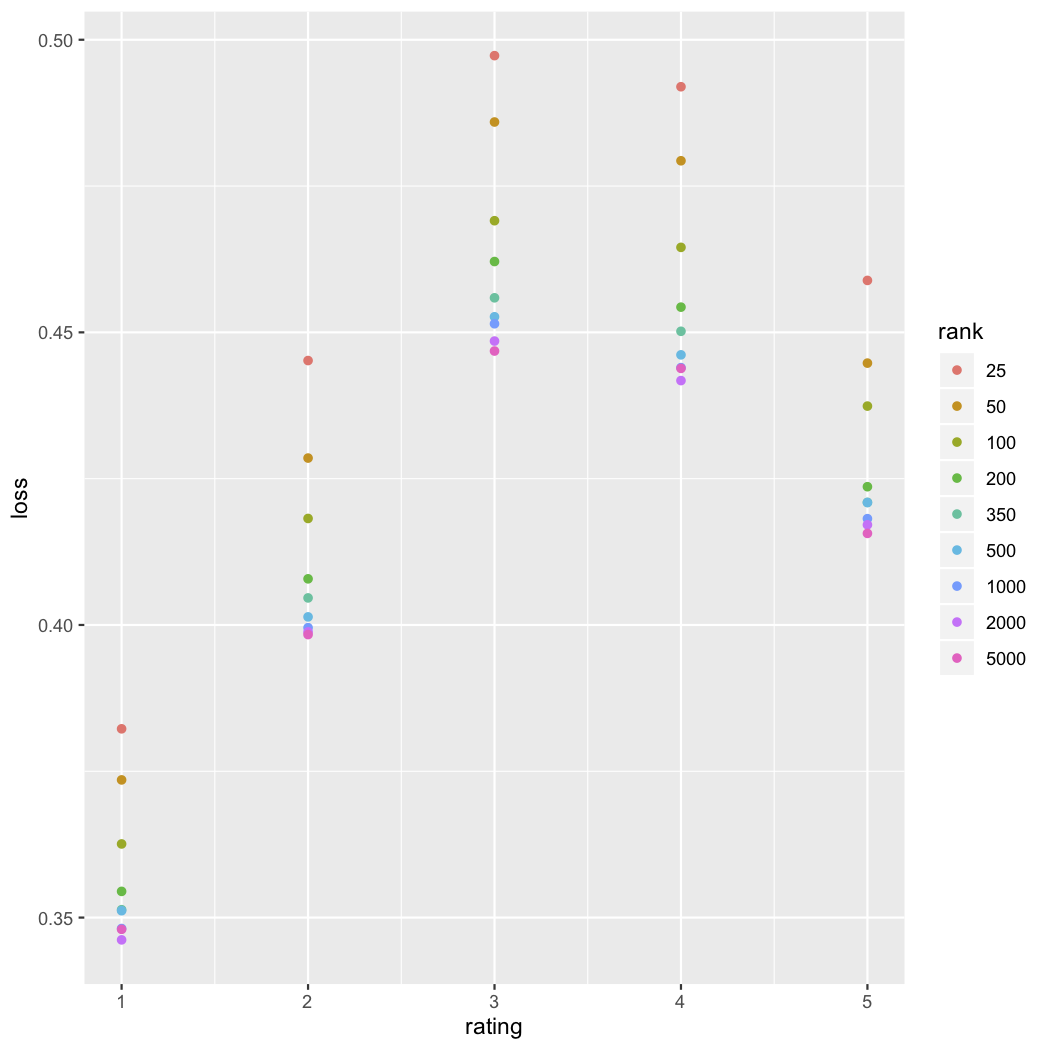
\includegraphics[width=\linewidth]{..\Graphs\FinalNMFMovie.png}
  \caption{MovieLens Rank x Loss}
\end{figure}

\begin{figure}
  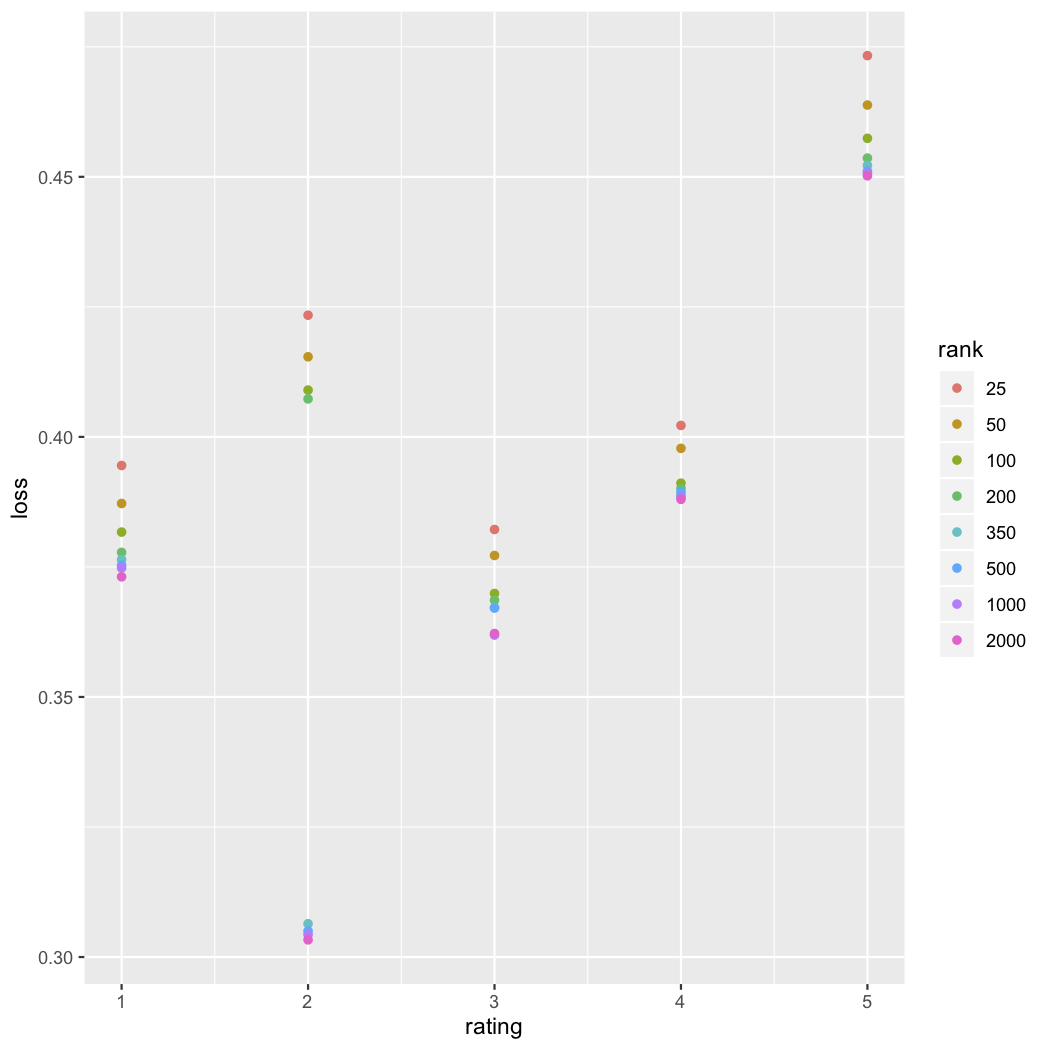
\includegraphics[width=\linewidth]{..\Graphs\FinalNMFSong.png}
  \caption{SongList Rank x Loss}
\end{figure}


As you can see the loss value continued to drop. Unfortunately, it was not able to run long enough to get higher rank value. Though we can see that change in loss begins to get very small and that likely we were close to the optimal rank.


\section{KNN - k Nearest Neighbors}

\section{CART - Classification and Regression Trees}

\section{Prediction Methods Comparisons}

\section{Helper Functions}
\subsection{embedDataMeans}
In certain data sets, it would be difficult to perform predictions directly. There are data sets where the item IDs are not ordinal, hence they don't have underlying ordering. The solution is to create dummy variables for these IDs until moving forward to testing them one at a time. 
For example, say we're using CART as our prediction method and there is a possibility that there would be at most one data point that satisfied two conditions, this creates issues when making trees. Rather than using minsplit, we can embed the user ID and item ID to do dimension reduction. In this function, our goal was to create a new data frame, that includes the mapping between the userID and its mean ratings, as well as the itemID and its mean ratings. 

\subsection{dataToMatrix} 
The goal of this function is to make data handling for KNN and NMF easier. This functions turns our data frame into a data table, and creates a matrix like form of data with the userID's corresponding rating to itemID. With this function, the entries are replaced with NA if the user has not rated the item. 

\newpage
\section{Who Did What}
\subsection{Leo}

\subsection{Ynna}

\subsection{Duong}

\subsection{Tycho}

\subsection{Jessica}

\newpage
\appendix
\section{TermProject.R}

\section{Probability Distributions Chart Generator}
For detailed comments, visit the repository
/ynnalecitona/ecs189g-termproject.
\begin{lstlisting}[language=R]
library(ggplot2)
library(reshape)
generate_distributions <- function(data_to_plot) {
data_to_plot[] <- lapply(data_to_plot, unlist)
data_to_plot <- melt(data_to_plot)
names(data_to_plot) <- c("ratings", "probabilities")
distribution_plot <- ggplot(data_to_plot, 
aes(ratings, probabilities, 
col= ratings)) + geom_point() + stat_smooth()
distribution_plot
}
\end{lstlisting}

\section {Experiment Sets Generator}
For detailed comments, visit the repository
/ynnalecitona/ecs189g-termproject.
\begin{lstlisting}[language = R]
does_contain_all <- function(targetList, checkList)
{
    numElementsLacked <- sum(!(checkList %in% targetList))
    return(numElementsLacked == 0)
}
sampling_data <- function(dataIn, sampleSize, 
verbose = FALSE) 
{
    if (sampleSize > nrow(dataIn)) {
        print("Error: Sample size greater than data size")
        return(-1)
    }
    uniqueUsersTotal <- unique(dataIn[,1])
    uniqueItemsTotal <- unique(dataIn[,2])
    samplingIdx <- sample(1:nrow(dataIn), sampleSize)
    sampleData <- dataIn[samplingIdx,]
    i <- 1
    while (!does_contain_all(sampleData[,1], 
    uniqueUsersTotal) || !does_contain_all(sampleData[,2], 
    uniqueItemsTotal)) {
        samplingIdx <- sample(1:nrow(dataIn), sampleSize)
        sampleData <- dataIn[samplingIdx,]
        i <- i + 1
    }
    if (verbose) {
        print("Trials needed: ")
        print(i)
    }
    return(sampleData)
}

create_experiment_sets <- function(dataIn, ratio)
{
    if (sum(ratio) != 1) {
        print("Invalid ratios")
        return(-1)
    }

    trainSetSize <- floor(nrow(dataIn) * ratio[1])
    validationSetSize <- floor(nrow(dataIn) * ratio[2])
    testSetSize <- nrow(dataIn) - trainSetSize 
    - validationSetSize

    trainSet <- sampling_data(dataIn, trainSetSize)
    print("Train set sampling done")

    sampledRows <- as.numeric(rownames(trainSet))
    leftovers <- dataIn[-sampledRows,]
    rownames(leftovers) <- 1:nrow(leftovers)

    samplingIdx <- sample(1:nrow(leftovers), 
    validationSetSize)
    validationSet <- leftovers[samplingIdx,]
    print("Validation set sampling done")

    sampledRows <- as.numeric(rownames(validationSet))
    testSet <- leftovers[-sampledRows,]
    print("Test set sampling done")

    experiment_sets <- list(trainSet = trainSet, 
    validationSet = validationSet, testSet = testSet)
    class(experiment_sets) <- "expSets"
    return(experiment_sets)
}

save_experiment_sets <- function(expSets)
{
    trainSet <- expSets$trainSet
    validationSet <- expSets$validationSet
    testSet <- expSets$testSet
    write.csv(trainSet, "train.data", row.names = FALSE)
    write.csv(validationSet, "validation.data", 
    row.names = FALSE)
    write.csv(testSet, "test.data", row.names = FALSE)
}

\end{lstlisting}

\section{Generate Partitions}
\begin{lstlisting}[language=R]
  test <- setdiff(1:nrow(dataIn), train)

  n <- floor(0.95 * nrow(dataIn))
  cond <- FALSE
  
  while(!cond) {

    trainIndx <- sample(nrow(dataIn), n)
    testIndx <- setdiff(1:nrow(dataIn), trainIndx)
    cond <- TRUE

    for(factor in names(dataIn)[1:2]) {
      trainLevels <- dataIn[trainIndx, factor]
      testLevels <- dataIn[testIndx, factor]
      
      if(!all(testLevels %in% trainLevels)) {
        cond <- FALSE
      }
    }
  }
\end{lstlisting}

\section{Aesthetic R Code in Latex}
https://tex.stackexchange.com/questions/374001/insert-r-code-in-latex

\section{Cross Validation with Factors}
https://stackoverflow.com/questions/19946930/r-cross-validation-

on-a-dataset-with-factors


\end{document}

